\chapter{KT Project: una panoramica} \label{chap:panoramica}

	In questo capitolo introdurremo i principali obiettivi del Progetto KT per Indico in modo da dare una panoramica generale dei sotto-progetti di cui il progetto principale è composto. Inoltre verranno esposti i principali strumenti e linguaggi utilizzati durante lo sviluppo del progetto.
	
	\section{Progetti principali} \label{sec:p;progetti_principali}
    	
    	Il progetto finanziato dal gruppo \ac{KT} per Indico, oggetto principale del programma di Technical Student a cui ha partecipato il sottoscritto, è nato come co-progetto tra i gruppi \ac{IT} e \ac{KT}. L'obiettivo principale di questo progetto era quello di migliorare la visibilità e l'impatto di Indico in tutto il mondo, in particolare al di fuori della comunità \acr{HEP}, all'interno della quale Indico si è già ampiamente affermato.
    	
    	Come si è già accennato nel Capitolo \ref{chap:CERN}, il concetto di \ac{KT} si basa sull'idea della diffusione e condivisione della conoscenza e degli strumenti necessari per ottenerla. L'idea alla base del progetto era quindi quella di modificare e migliorare il software Indico in modo da permettere una miglior diffusione dello stesso nel mondo. Per fare questo, il KT Project si era prefissato tre obiettivi generali da raggiungere:
    	
    	\begin{itemize}
        	\item rendere Indico più accessibile agli utenti
        	\item rendere Indico più semplice da utilizzare e personalizzare
        	\item rendere Indico, in generale, più moderno e visivamente ``attraente''
    	\end{itemize}
    	
    	Gli obiettivi prefissati col Progetto KT erano quindi molto ampi e generali e, come ci può immaginare, anche piuttosto complessi da mettere in pratica. Per questa ragione il progetto che è stato assegnato al sottoscritto non era che il primo di una serie di progetti, finanziati dal gruppo \ac{KT}, al fine di migliorare l'impatto a livello mondiale del software Indico. Infatti, durante il periodo dei 14 mesi passati a Ginevra dal sottoscritto, erano stati approvati e finanziati già due progetti dal gruppo \ac{KT} per Indico: il primo, assegnato al sottoscritto, ed un secondo da assegnare ad un futuro membro del team Indico, molto probabilmente un altro Techical Student.
    	
    	Il primo Progetto KT per Indico è stato quindi pianificato e suddiviso in una serie di sotto-progetti, i quali dovevano essere terminati durante i 12 (poi diventati 14) mesi del programma Technical Student (si veda \cite{pedro:gist} per la prima stesura del progetto). Quattro di questi sotto-progetti sono risultati essere più importanti e complessi degli altri e sono andati ad occupare la maggior parte del periodo di Technical Student. Di seguito ne parleremo brevemente per avere un'idea generale dei progetti principali del KT Project, mentre nei Capitoli successivi vedremo in dettaglio ognuno di essi.
    	
    	\subsection{Cloud Deployment} \label{subsec:p;pp;cloud}
    	
        	La prima fase del Progetto KT riguardava il Cloud Deployment di Indico, ovvero l'automatizzazione del processo di installazione e configurazione di Indico sia in ambiente cloud che in ambiente virtuale.
        	
        	Il progetto è durato circe un mese e mezzo, dal 23 Ottobre al 9 Dicembre 2013, ed ha portato alla stesura di due script fabric, uno per la creazione di immagini virtuali ed uno di gestione remota, ed una recipe cloud-init, per il deployment su struttura cloud.
    	
    	\subsection{Distribuzione e Packaging} \label{subsec:p;pp:distribuzione}
    	
        	Il secondo progetto del KT Project riguardava invece Distribuzione e Packaging, ovvero l'automatizzazione della creazione di diverse distribuzioni di Indico, sia dei sorgenti che precompilate, basate su diverse versioni sia di Indico che di Python e, successivamente, il caricamento di queste distribuzioni su un server e su GitHub.
        	
        	Questo progetto è durato circa due settimane, dal 27 Gennaio all'11 Febbraio 2014 ed il risultato è stato lo sviluppo di uno script fabric che automatizza l'intero processo di distribuzione.
    	
    	\subsection{Instance Tracking} \label{subsec:p;pp;instance_tracker}
    	
        	Il progetto sull'Instance Tracking si occupava invece di sviluppare un'applicazione web stand-alone per il tracciamento delle istanze di Indico e la successiva analisi statistica delle informazioni raccolte.
        	
        	Questo progetto, tra tutti, si è dimostrato essere il più importante, richiedendo 4 mesi di sviluppo, dall'11 Febbraio al 10 Giugno 2014. Il risultato di questo progetto è stato lo sviluppo di un'applicazione di tracciamento, successivamente denominata ``Cephalopod''.
    	
    	\subsection{Conference Customization Prototype} \label{subsec:p;pp;conference_customization_prototype}
    	
        	L'ultimo progetto era incentrato invece sullo sviluppo di un prototipo che aiutasse il team di Indico a decidere come sviluppare, in futuro, una nuova versione del tool per la personalizzazione delle conferenze.
        	
        	Sebbene non molto incisivo dal punto di vista dello sviluppo, quest'ultimo progetto è risultato molto impegnativo in quanto è stato caratterizzato da continui cambi di programma e frequenti sessioni di brainstorming con l'intero team di sviluppo. Quest'ultima fase è durata in totale circa 5 e mezzo, dal 10 Giugno a fine Novembre 2014.
    	
    \section{Strumenti e linguaggi} \label{sec:p;strumenti_linguaggi}
    
        Con questa ultima Sezione introduttiva, intendiamo fornire al lettore una serie di conoscenze e nozioni di base utili a capire il lavoro svolto con questo progetto. Indico infatti è composto da molti linguaggi diversi ed utilizza molti strumenti, sviluppati da terzi, senza i quali non potrebbe funzionare. È necessario quindi sapere quali sono e cosa fanno ognuno di questi strumenti, nonché essere a conoscenza dei linguaggi utilizzati.
        
        \subsection{GitHub} \label{subsec:p;sl;github}
        
            GitHub è un servizio web per l'hosting di repository Git\footnote{Git è un noto sistema per la gestione del codice e lo sviluppo di applicazioni sviluppato da Linus Torvalds.}. Github offre le funzionalità caratteristiche di Git, come controllo di versione distribuito o gestione del codice sorgente. Tuttavia, a differenza di Git che è soltanto uno strumento da linea di comando, Github offre un'interfaccia grafica basata sul web. Inoltre fornisce molte funzionalità incentrate sulla collaborazione di più sviluppatori, come tracciamento dei bug, richiesta di funzionalità, gestione delle attività e pagine wiki per ogni progetto.
            
        	\begin{figure}[h!]
        		\begin{center}
        			
\includegraphics[scale=0.2]{octocat.png}
        		\end{center}
        		\caption[Octocat]{Octocat, la mascotte ufficiale di GitHub.}
        		\label{fig:octocat}
        	\end{figure}
        	
        	GitHub offre opzioni sia per repository privati, a pagamento, che pubblici, completamente gratuiti. Quest'ultimi vengono solitamente utilizzati per ospitare progetti software open source, come nel caso di Indico.
        	
        	In GitHub si possono creare profili utente, al quale si accede tramite delle credenziali, o organizzazioni, che rappresentano la collaborazione di più individui. Ogni utente e ogni organizzazione può definire una serie di repository, pubblici o privati, condivisi o meno. La pagina GitHub dell'organizzazione Indico è ad esempio \url{https://github.com/indico}, mentre quella del sottoscritto \url{https://github.com/oddlord}. La pagina GitHub di Indico ospita molti progetti, tutti legati a Indico, ma che non sono necessariamente il progetto Indico principale: ad esempio il repository del progetto principale Indico si trova all'indirizzo \url{https://github.com/indico/indico}, mentre il progetto sul Cloud Deployment sviluppato dal sottoscritto è all'indirizzo \url{https://github.com/indico/indico-cloud-images}.
    
        \subsection{Python} \label{subsec:p;sl;python}
        
            Python è un linguaggio di programmazione dinamico, di alto livello, general-purpose e interpretato che, al momento, è molto diffuso e utilizzato, specialmente nel settore delle applicazioni web. La filosofia di Python tende a enfatizzare la leggibilità del codice, proponendo una sintassi tramite la quale il programmatore può scrivere programmi anche in poche linee di codice, cosa che sarebbe impossibile con linguaggi come C++ o Java. \cite{wiki:python}
        
        	\begin{figure}[h!]
        		\begin{center}
        			
\includegraphics[scale=0.6]{python_logo.png}
        		\end{center}
        		\caption[Logo di Python]{Logo di Python.}
        		\label{fig:python_logo}
        	\end{figure}
        	
        	Python supporta molti paradigmi di programmazione, tra i quali programmazione a oggetti, imperativa e funzionale/procedurale. Il sistema di tipaggio di Python è dinamico, ovvero la correttezza dei tipi dei vari oggetti viene stabilita in tempo di esecuzione.
        	
        	Indico è un software principalmente scritto in Python. Per questo motivo all'interno di questa tesi faremo riferimento spesso l'utilizzo di comandi o librerie Python, per descrivere lo sviluppo dei vari progetti che hanno composto il KT Project.
        
            Un importante comando offerto da Python è \python{.format()}, che sarà accennato all'interno del Capitolo \ref{chap:cloud_deployment}. Questa funzione sostituisce a degli speciali \textit{placeholder} (o segnaposti, in italiano), presenti nell'oggetto stringa sul quale viene eseguito, i valori associati ad ogni placeholder tramite un particolare dizionario, passato come unico argomento. I placeholder sono parole chiave che identificano un parametro in modo univoco racchiuse tra parentesi graffe. Il comando \python{.format()} funziona quindi come segue:
            
            \begin{center}
                \begin{lstlisting}[language=python, gobble=18]
                    data = {'first': 'Hodor', 'last': 'Hodor!'}
                    template = '{first} {last}'
                    result = template.format(**data)
                \end{lstlisting}
                \captionsetup{textformat=empty,labelformat=empty} \vspace{-2em}
                \captionof{lstlisting}[Comando \python{.format()} (esempio)]{Esempio del funzionamento del comando \python{.format()}.}
            \end{center}
            
            Il risultato salvato in \python{result} sarà quindi la stringa \python{'Hodor Hodor!'}.
        
        \subsection{Cloud-init} \label{subsec:p;sl;cloud-init}
        
            Cloud-init\footnote{\url{https://launchpad.net/cloud-init}.} è uno degli strumenti più utilizzati per l'inizializzazione e configurazione di server cloud. Tramite la compilazione di alcune semplici impostazioni, l'utente sarà in grado di avviare un nuovo server cloud specificando una serie di azioni da eseguire in automatico durante il primo avvio, come ad esempio eseguire determinati script, copiare alcuni file da remoto, installare pacchetti ed applicazioni necessarie, e così via. Cloud-init è installato di default su molte distribuzioni Linux, come Ubuntu, Fedora, Debian, CentOS, ecc. \cite{cloud-init:readthedocs}
            
            In poche parole, Cloud-init è un modulo che viene eseguito all'avvio di una macchina virtuale e permette di specificare delle azioni da eseguire tramite un file detto \textit{user-data}. Un file di questo tipo, ovvero che permette di specificare una serie di azioni che verranno eseguite in automatico, viene detto \textit{recipe} (ovvero ``ricetta'' in inglese). Si parla infatti di \textit{cloud-init recipe} riferendosi ad una particolare configurazione da passare a cloud-init.
            
            Per utilizzare una cloud-init recipe, è sufficiente specificare il file \bash{user-data} generato quando si avvia il server sul cloud per la prima volta. Il comando da usare varia a seconda del Cloud Service Provider scelto. Per infrastrutture cloud basate su tecnologia OpenStack, ad esempio, è sufficiente eseguire il seguente comando da terminale:
            
            \begin{center}
                \begin{lstlisting}[language=bash, gobble=18]
                    $ nova boot --image ubuntu-cloudimage --flavor 1 --user-data user-data
                \end{lstlisting}
                \captionsetup{textformat=empty,labelformat=empty} \vspace{-2em}
                \captionof{lstlisting}[Boot con cloud-init (esempio OpenStack)]{Esempio di comando di boot con cloud-init per infrastrutture basate su OpenStack.}
            \end{center}
            
            Tramite il file \bash{user-data} è possibile passare al modulo cloud-init una serie di file in diversi formati supportati, tra i quali:
            
            \begin{itemize}
                \item file compresso in formato \bash{.gzip};
                \item file \acr{MIME} multiparti;
                \item script bash;
                \item file cloud-config.
            \end{itemize}
            
            In particolare, i file gzip possono essere utili per ridurre le dimensioni del file \bash{user-data}, essendo questo limitato a 16KB. I file \ac{MIME} multiparti sono tipi di file composti che servono a raggruppare altri file, dei tipi sopra citati, in un unico file. I file di script servono ad eseguire una serie di comandi subito dopo il primo boot, mentre i file cloud-config sono particolari file utilizzati per copiare file in remoto sulla macchina sul cloud oppure per installare tutti i pacchetti aggiuntivi necessari.
            
            Come vedremo nel Capitolo \ref{chap:cloud_deployment}, le recipe cloud-init sono state molto utili per la fase di Cloud Deployment di Indico.
                    
        \subsection{Fabric} \label{subsec:p;sl;fabric}
        
            Fabric è una ``libreria Python e uno strumento da linea di comando per rendere più semplice l'uso di \acr{SSH} per applicazioni di deployment o operazioni di amministrazione di sistema''. \cite{fabric:documentation}
            
        	\begin{figure}[h!]
        		\begin{center}
        			
\includegraphics[scale=1]{fabric_logo.png}
        		\end{center}
        		\caption[Logo di Fabric]{Logo di Fabric.}
        		\label{fig:fabric_logo}
        	\end{figure}
            
            Fabric fornisce una serie di comandi per l'esecuzione sia locale che remota di comandi shell (normali o tramite \bash{sudo}), per l'upload o il download di file o per l'esecuzione di operazioni ausiliare, come richiedere un input all'utente o bloccare l'esecuzione di un'operazione in esecuzione.
            
            Uno script fabric è quindi un semplice script python, dove però si possono utilizzare tutti i comandi messi a disposizione da Fabric. Due comandi fabric molto importanti sono \python{local(cmd)} e \python{run(cmd)}. Entrambi i comandi eseguono il comando \python{cmd} passato come argomento come comando shell, l'unica differenza tra i due è che \python{local(cmd)} esegue \python{cmd} in locale, ovvero sulla macchina che sta eseguendo lo script fabric, mentre \python{run(cmd)} esegue \python{cmd} su una macchina remota, opportunamente specificata. Inoltre un altro comando molto utile è il comando \python{put(file, dest)} che permette di copiare il file \python{file}, che si trova sulla macchina locale, nella destinazione \python{dest} all'interno della macchina remota, quindi mimando il comportamento del comando \bash{scp} di bash.
            
            Per permettere una stesura più semplice e meno ridondante di uno script fabric, è possibile specificare alcune opzioni in un particolare dizionario, detto \textit{ambiente} e denotato dalla variabile \python{env}, in modo da non doverle ripetere ogni volta che si invoca un comando fabric. Ad esempio specificando un valore per il campo \python{env.hosts} possiamo definire una volta per tutte l'indirizzo di tutte le macchine remote su cui vogliamo eseguire i comandi passati a \python{run()}, senza dover stare a ripeterli inutilmente ogni volta.
            
            Ogni script fabric deve specificare delle operazioni, dette \textit{task}, che possono poi essere eseguite da linea di comando. Ogni task è una funzione python contrassegnata dal decoratore \python{@task}, che contraddistingue le task (operazioni che possono essere eseguite dall'utente) da funzioni interne dello script.
            
            Per poter essere eseguito, uno script fabric deve essere chiamato \bash{fabfile.py}. Per eseguire quindi uno script fabric basta eseguire un comando della forma seguente:
            
            \begin{center}
                \begin{lstlisting}[language=bash, gobble=18]
                    $ fab task1 task2
                \end{lstlisting}
                \captionsetup{textformat=empty,labelformat=empty} \vspace{-2em}
                \captionof{lstlisting}[Esecuzione task fabric (esempio)]{Esempio dell'esecuzione di due task fabric.}
            \end{center}
            
            Un comando come quello appena mostrato esegue prima la task \bash{task1} e quindi \bash{task2} definite nel file \bash{fabfile.py}.
            
            Fabric verrà utilizzato, all'interno del progetto di Cloud Deployment, per la stesura sia di uno script per la creazione automatica di immagini virtuali che di uno script per la gestione remota di macchine cloud. Inoltre sarà utilizzato anche per la fase di Distribuzione e Packaging.
        
        \subsection{QEMU e KVM} \label{subsec:p;sl;qemu_kvm}
        
            \acr{QEMU} è un emulatore e strumento di virtualizzazione open source. \acr{KVM} invece è anch'esso uno strumento di virtualizzazione e fornisce anche delle funzionalità di accelerazione hardware per sistemi Linux.
            
            \ac{QEMU} e \ac{KVM} possono essere utilizzati in congiunzione, tant'è che \ac{KVM} viene distribuito da anni assieme a \ac{QEMU}. Si potrebbe pensare di utilizzare soltanto uno di questi due strumenti per lavorare con macchine virtuali, tuttavia, anche se \ac{QEMU} fornisce un sistema di virtualizzazione completo e a se stante, per applicazioni pratiche è spesso necessario affiancargli \ac{KVM} per migliorarne le performance. D'altro canto, \ac{KVM} soltanto non fornisce tutte le funzionalità di un ambiente di virtualizzazione completo come \ac{QEMU}.
            
            \ac{QEMU} e \ac{KVM} sono stati utilizzati durante la fase di Cloud Deployment del progetto, ed in particolare nello script di creazione di immagini virtuali, come vedremo all'interno del Capitolo \ref{chap:cloud_deployment}.
            
            Per maggiori informazioni su \ac{QEMU} e \ac{KVM} si consultino \cite{kvm:wiki} e \cite{qemu:wiki}.
        
        \subsection{Requests} \label{subsec:p;sl;requests}
        
            Requests è una delle più semplici, in termini di utilizzo, librerie \acr{HTTP} per Python.
            
            Grazie a Requests si possono fare richieste, o inviare dati, tramite il protocollo \ac{HTTP} scrivendo solo poche linee di codice, in piena filosofia Python. Se ad esempio volessimo ottenere la lista degli eventi pubblici di GitHub, basterebbe scrivere la seguente linea di codice:
            
            \begin{center}
                \begin{lstlisting}[language=python, gobble=18]
                    r = requests.get('https://api.github.com/events')
                \end{lstlisting}
                \captionsetup{textformat=empty,labelformat=empty} \vspace{-2em}
                \captionof{lstlisting}[\python{get()} con Requests (esempio)]{Esempio del comando \python{get()} della libreria Requests.}
            \end{center}
            
            All'interno della variabile \python{r} sarà quindi presente la risposta ottenuta dall'esecuzione di quella richiesta. La risposta ad una richiesta può essere di svariati tipi e solitamente contiene tutti i dati richiesti, opportunamente strutturati. Nell'esempio di sopra la risposta sarà in formato \acr{JSON}.
            
            L'esempio opposto riguarda invece l'invio di dati tramite un'\ac{API}. Per inviare dei dati basta semplicemente utilizzare il comando \python{post()}, come mostrato dall'esempio seguente:
            
            \begin{center}
                \begin{lstlisting}[language=python, gobble=18]
                    r = requests.post('http://httpbin.org/post', data = {'key':'value'})
                \end{lstlisting}
                \captionsetup{textformat=empty,labelformat=empty} \vspace{-2em}
                \captionof{lstlisting}[\python{post()} con Requests (esempio)]{Esempio del comando \python{post()} della libreria Requests.}
            \end{center}
            
            Requests verrà utilizzata ampiamente all'interno del progetto di Instance Tracking (Capitolo \ref{chap:instance_tracker}) e anche durante la fase di upload a GitHub del progetto di Distribuzione e Packaging (Capitolo \ref{chap:distribuzione_packaging}).
        
        \subsection{Twitter Bootstrap} \label{subsec:p;sl;twitter_bootstrap}
        
            Bootstrap\footnote{\url{http://getbootstrap.com/}.}, sviluppato da Twitter, è uno dei più famosi framework \ac{HTTP}, \acr{CSS} e Javascript per sviluppare progetti web dinamici e reattivi e dal design moderno.
            
            Scaricando i file di Bootstrap ed includendoli nel progetto, uno sviluppatore web ha accesso a tutta una serie di stili, elementi \acr{HTML} e funzioni Javascript che gli permettono, in poche linee di codice, di creare da zero un sito dinamico e moderno.
            
            Bootstrap, ad esempio, include un set di icone, dette Glyphicons, dallo stile minimalista e gradevole. Tramite il codice seguente, ad esempio, si produce il bottone in Figura \ref{fig:button_bootstrap}.
            
            \begin{center}
                \begin{lstlisting}[language=html, gobble=18]
                    <button type="button" class="btn btn-default btn-lg">
                        <span class="glyphicon glyphicon-star" aria-hidden="true"></span> Star
                    </button>
                \end{lstlisting}
                \captionsetup{textformat=empty,labelformat=empty} \vspace{-2em}
                \captionof{lstlisting}[Bottone con Bootstrap (esempio)]{Esempio della definizione di un bottone con icona con Bootstrap.}
            \end{center}
            
        	\begin{figure}[h!]
        		\begin{center}
        			
\includegraphics[scale=1]{button_bootstrap.png}
        		\end{center}
        		\caption[Bottone con Bootstrap (esempio)]{Esempio di un bottone con icona con Bootstrap.}
        		\label{fig:button_bootstrap}
        	\end{figure}
        	
        	Un bottone così definito risulta avere uno stile dinamico, ad esempio diventa ombreggiato al passaggio del mouse e rientra quando viene cliccato.
        	
        	Un altro esempio possono essere i menu a tendina. Tramite il frammento di codice \ac{HTML} seguente, ad esempio, si genera un menu a tendina come in Figura \ref{fig:dropdown_bootstrap}.
        	
        	
            \begin{center}
                \begin{lstlisting}[language=html, gobble=18]
                    <div class="dropdown">
                        <button class="btn btn-default dropdown-toggle" type="button" id="dropdownMenu1" data-toggle="dropdown" aria-haspopup="true" aria-expanded="true">
                            Dropdown
                            <span class="caret"></span>
                        </button>
                        <ul class="dropdown-menu" aria-labelledby="dropdownMenu1">
                            <li><a href="#">Action</a></li>
                            <li><a href="#">Another action</a></li>
                            <li><a href="#">Something else here</a></li>
                            <li role="separator" class="divider"></li>
                            <li><a href="#">Separated link</a></li>
                        </ul>
                    </div>
                \end{lstlisting}
                \captionsetup{textformat=empty,labelformat=empty} \vspace{-2em}
                \captionof{lstlisting}[Menu a tendina con Bootstrap (esempio)]{Esempio della definizione di un menu a tendina con Bootstrap.}
            \end{center}
            
        	\begin{figure}[h!]
        		\begin{center}
        			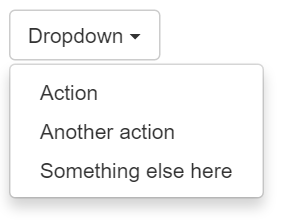
\includegraphics[scale=1]{dropdown_bootstrap.png}
        		\end{center}
        		\caption[Menu a tendina con Bootstrap (esempio)]{Esempio di un menu a tendina con Bootstrap.}
        		\label{fig:dropdown_bootstrap}
        	\end{figure}
        	
        	Bootstrap sarà utilizzato come stile di base per l'applicazione sviluppata durante il progetto di Instance Tracking, descritto all'interno del Capitolo \ref{chap:instance_tracker}.
        
        \subsection{Flask} \label{subsec:p;sl;flask}
        
            Flask\footnote{\url{http://flask.pocoo.org/}.} è un microframework per sviluppare applicazioni web in Python basato su Werkzeug e Jinja2.
            
            Un esempio minimale di applicazione è il frammento di codice seguente, che immaginiamo essere memorizzato all'interno del file \bash{hello.py}:
            
            \begin{center}
                \begin{lstlisting}[language=python, gobble=18]
                    from flask import Flask
                    app = Flask(__name__)
                    
                    @app.route("/")
                    def hello():
                        return "Hello World!"
                    
                    if __name__ == "__main__":
                        app.run()
                \end{lstlisting}
                \captionsetup{textformat=empty,labelformat=empty} \vspace{-2em}
                \captionof{lstlisting}[Applicazione in Flask (esempio)]{Esempio della definizione di un'applicazione con Flask.}
            \end{center}
            
            L'applicazione può quindi essere avviata eseguendo la seguente istruzione da linea di comando:
            
            \begin{center}
                \begin{lstlisting}[language=bash, gobble=18]
                    $ python hello.py
                     * Running on http://localhost:5000/
                \end{lstlisting}
                \captionsetup{textformat=empty,labelformat=empty} \vspace{-2em}
                \captionof{lstlisting}[Esecuzione dell'applicazione in Flask (esempio)]{Esempio di esecuzione dell'applicazione con Flask.}
            \end{center}
            
            Quindi, accedendo all'\ac{URL} \html{http://localhost:5000/}, si vedrà stampata sul browser la stringa \html{Hello World!}.
            
            Flask mette a disposizione dello sviluppatore delle funzioni molto importanti, ad esempio per fare \textit{\ac{URL} routing} o \textit{template rendering}. L'azione di associare un \ac{URL} ad una funzione è detto \ac{URL} routing (ovvero ``indirizzamento degli \ac{URL}'') ed è resa disponibile grazie al decoratore di Flask \python{route()}. Una volta associato l'\ac{URL} alla funzione desiderata, la funzione può eseguire i comandi specificati ogni volta che si accede a tale \ac{URL}. In particolare, se l'\ac{URL} corrisponde alla visualizzazione di una pagina, allora tale funzione dovrà occuparsi di generare la pagina richiesta e quindi restituirla, utilizzando la funzione Flask \python{render_template()}. Il comando \python{render_template()} prende in input un file di template, scritto in Jinja2, ed un dizionario di variabili e restituisce il file istanziato, ovvero il template a cui sono stati sostituiti i valori dei parametri ai placeholder presenti nel template, in modo molto simile a quanto visto per \python{format()}. Inoltre, Flask mette a disposizione altre funzioni utili, come ad esempio la funzione \python{redirect()}, che serve a reindirizzare l'applicazione su un altro \ac{URL}, oppure il decoratore \python{login_required}, che permette di eseguire i comandi di una certa funzione se e solo se si chi richiede l'\ac{URL} è un utente correttamente registrato e loggato, restituendo altrimenti un errore.
            
            Flask è stato utilizzato come framework per Cephalopod, l'applicazione descritta all'interno del Capitolo \ref{chap:instance_tracker}, e per il prototipo sviluppato per la fase di Conference Customization (Capitolo \ref{chap:conference_customization_prototype}).
            
        \subsection{Jinja2} \label{subsec:p;sl;jinja2}
        
            Jinja2 è un template engine molto diffuso per Python compatibile con Flask.
            
            Uno dei vantaggi di Jinja2 è la possibilità di definire blocchi condizionali e cicli all'interno del template. Prendiamo ad esempio il seguente frammento di template scritto in sintassi Jinja2:
            
            \begin{center}
                \begin{lstlisting}[language=html, gobble=18]
                    <ul>
                        
                            <li><a href="{{ user.url }}">{{ user.username }}</a></li>
                        
                    </ul>
                \end{lstlisting}
                \captionsetup{textformat=empty,labelformat=empty} \vspace{-2em}
                \captionof{lstlisting}[Template in Jinja2 (esempio)]{Esempio della definizione di un template con Jinja2.}
            \end{center}
            
            Consideriamo quindi il seguente dizionario Python:
            
            \begin{center}
                \begin{lstlisting}[language=python, gobble=18]
                    {
                        'users': [
                            {'username': 'Tommy', 'url': 'www.tommy.com'},
                            {'username': 'Doge', 'url': 'www.dogetheking.org'},
                            {'username': 'The Guy', 'url': 'www.theguy.co.uk'}
                        ]
                    }
                \end{lstlisting}
                \captionsetup{textformat=empty,labelformat=empty} \vspace{-2em}
                \captionof{lstlisting}[Dizionario di parametri per il template (esempio)]{Esempio di dizionario di parametri per istanziare il template.}
            \end{center}
            
            Quindi, se a questo punto invochiamo il comando \python{render_template()} di Flask sul template e la lista appena definiti, otteniamo il seguente frammento di codice \ac{HTML}, che rappresenta l'istanziazione del template secondo i parametri passati:
            
            \begin{center}
                \begin{lstlisting}[language=html, gobble=18]
                    <ul>
                        <li><a href="www.tommy.com">Tommy</a></li>
                        <li><a href="www.dogetheking.org">Doge</a></li>
                        <li><a href="www.theguy.co.uk">The Guy</a></li>
                    </ul>
                \end{lstlisting}
                \captionsetup{textformat=empty,labelformat=empty} \vspace{-2em}
                \captionof{lstlisting}[Template in Jinja2 (esempio)]{Esempio della definizione di un template con Jinja2.}
            \end{center}
            
            Jinja2, in congiunzione con Flask, è stato utilizzato per lo sviluppo di Cephalopod, come vedremo all'interno del Capitolo \ref{chap:instance_tracker}.
        
        \subsection{PostgreSQL e SQLAlchemy} \label{subsec:p;sl;postgreSQL_SQLAlchemy}
        
            PostgreSQL\footnote{\url{http://www.postgresql.org/}.} è un potente database \acr{ORDBMS}, ovvero relazionale orientato a oggetti, open source. In commercio da più di 15 anni, PostgreSQL è disponibile per tutti i maggiori sistemi operativi, tra i quali Linux, Unix e Windows. Indico, al momento, utilizza un sistema di database ibrido, utilizzando sia \ac{ZODB} che PostgreSQL, migrando piano piano tutto il database su quest'ultimo.
            
        	\begin{figure}[h!]
        		\begin{center}
        			
\includegraphics[scale=0.5]{postgresql_logo.png}
        		\end{center}
        		\caption[Logo di PostgreSQL]{Logo di PostgreSQL.}
        		\label{fig:postgresql_logo}
        	\end{figure}
        	
        	SQLAlchemy\footnote{\url{http://www.sqlalchemy.org/}.}, invece, è un toolkit \acr{SQL} per Python, ovvero uno strumento che permette ad applicazioni Python di comunicare con database \ac{SQL}. Per maggiori informazioni sul supporto di SQLAlchemy a PostgreSQL si veda \cite{sqlalchemy:postgresql}.
        	
        	L'accoppiata PostgreSQL-SQLAlchemy è stata utilizzata per sviluppare Cephalopod, il tracciatore d'istanze descritto all'interno del Capitolo \ref{chap:instance_tracker}.
        
        \subsection{jqPlot} \label{subsec:p;sl;jqplot}
        
            jqPlot\footnote{\url{http://www.jqplot.com/}.} è un plugin Javascript per la visualizzazione di grafici. jqPlot permette di definire grafici interattivi e dinamici ed offre allo sviluppatore la possibilità di personalizzare ogni grafico tramite una vasta scelta di stili disponibili. Tra gli stili più noti troviamo il grafico a barre, il grafico a linea e il grafico a torta. Ad ogni grafico possono essere inoltre associate una serie di opzioni, per definirne l'aspetto ed il comportamento. Ci sono opzioni, ad esempio, per attivare o meno l'animazione del grafico, o per visualizzare delle etichette sui vari punti del grafico, o ancora per definire nuovi punti del grafico semplicemente cliccando col mouse.
            
            Il codice d'esempio seguente mostra quanto sia facile definire, con jqPlot, un grafico come quello in Figura \ref{fig:jqplot}.
            
            \begin{center}
                \begin{lstlisting}[language=javascript, gobble=18]
                    $(document).ready(function(){
                        var plot1 = $.jqplot ('chart1', [[3,7,9,1,5,3,8,2,5]]);
                    });
                \end{lstlisting}
                \captionsetup{textformat=empty,labelformat=empty} \vspace{-2em}
                \captionof{lstlisting}[Grafico con jqPlot (esempio)]{Esempio della definizione di un grafico a linea semplice con jqPlot.}
            \end{center}
            
        	\begin{figure}[h!]
        		\begin{center}
        			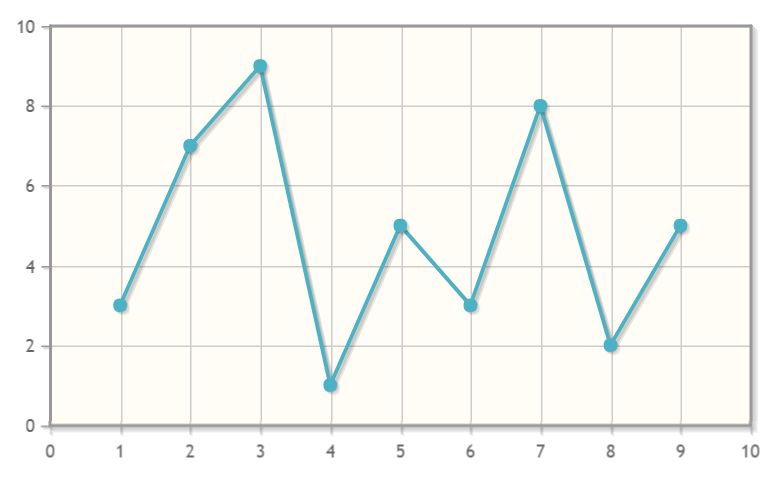
\includegraphics[scale=0.8]{jqplot.png}
        		\end{center}
        		\caption[Grafico con jqPlot (esempio)]{Esempio di un grafico a linea semplice con jqPlot (fonte \cite{jqplot:examples}).}
        		\label{fig:jqplot}
        	\end{figure}
        	
        	Per poter utilizzare le funzioni e gli stili offerti da jqPlot è sufficiente scaricare i sorgenti dal sito ufficiale di jqPlot, includerli all'interno della directory del progetto e quindi importare i file necessari all'interno del codice Javascript, che vogliamo produca il grafico, dell'applicazione che si sta sviluppando.
        	
        	jqPlot è stato utilizzato per sviluppare la pagina delle statistiche del tracciatore d'istanze (Capitolo \ref{chap:instance_tracker}) e per costruire la nuova pagina delle statistiche per Indico (Capitolo \ref{chap:altri_progetti}).
